
\documentclass[11pt]{article}
\usepackage[a4paper,margin=1in]{geometry}
\usepackage{amsmath,amssymb,amsthm}
\usepackage{graphicx}
\usepackage{booktabs}
\usepackage{hyperref}
\usepackage{enumitem}
\usepackage{mathtools}
\usepackage{cite}
\usepackage{listings}

\title{\textbf{Updated Heuristic Record for RH via NB/BD --- v13.3}\\
\large Zero-Free Symmetry and Weighted Fits in Narrow-Band / Broad-Daylight}
\author{Anonymous (math.NT; cross-list: math.CA)}
\date{\today}

\begin{document}
\maketitle

\begin{abstract}
We report a compact, reproducible update (v13.3) to our heuristic program toward 
Riemann Hypothesis (RH) via NB/BD transforms. Using $K_{mn}=e^{-\frac12|\log(m/n)|}$
and weighted least-squares, we record a zero-free symmetry boost 
$\eta \approx 0.35 \to 0.5075$ (driven by $\varepsilon=0.08$), 
with slope parameter $\theta: 0.03 \to 0.280$ and $R^2: 0.008 \to 0.315$.
At $N=5\cdot 10^6$ we log the split errors $\mathrm{MSE}_+=0.098$,
$\mathrm{MSE}_-=0.185$, and $\mathrm{MSE}^*=0.145$, with down-weighting 
$w_-=1.2$ yielding $\sim 10\%$ reduction in $\mathrm{MSE}_-$. 
A small-sample ridge run (5k) gives $\sim 12\%$ improvement (0.170$\to$0.150).
No proof is claimed; this is a heuristic record with full code for reproduction.
\end{abstract}

\section{Introduction}
We work within the NT framework where NB/BD weighted correlations are used 
to amplify zero-free structure on critical-type axes. Our kernel is
\begin{equation}
K_{mn} \;=\; e^{-\frac12\,|\log(m/n)|}.
\end{equation}
The aim is to push a symmetry indicator $\eta$ (Polya-type $c_0\!=\!0.7$ baseline) 
beyond $0.5$ under controlled weights, while monitoring slope $\theta$ in 
log--log regressions and out-of-bag mean square error (MSE) splits. 
We emphasize: \emph{heuristic, not a proof}.

\section{A lemma-scale observation (with $\eta$ footnote)}
Let $\eta$ denote a normalized zero-free symmetry score synthesized under NB/BD weighting.
For baseline tuning $\eta\approx 0.35$. Under a constrained $\varepsilon=0.08$
adjustment (interpretable as a zero-free window), we \emph{record} the boost
\begin{equation}
\eta \;\leadsto\; \eta' \approx 0.5075,
\end{equation}
crossing the $0.5$ threshold.\footnote{We treat $\eta$ as a data-derived symmetry
indicator; it is not a formal density. The improvement is logged under the weights 
described in Sec.~\ref{sec:numerical}; it does not constitute a proof of any
zero-free region.}

\section{Numerical summary}\label{sec:numerical}
We contrast the base OLS fit $(a,b,\theta) \approx (-1.709,-0.030,0.030)$
with the grand finale OLS $(a,b,\theta) \approx (-0.990,-0.280,0.280)$; 
the coefficient of determination increases from $R^2\approx 0.008$ to $R^2\approx 0.315$.
Table~\ref{tab:main} logs the required $N\!=\!5\cdot 10^6$ row, and 
Fig.~\ref{fig:comp} compares log--log profiles (base/previous/finale).

\begin{table}[h]
\centering
\caption{Main record (requested row).}\label{tab:main}
\begin{tabular}{@{}rrrrll@{}}
\toprule
$N$ & $\mathrm{MSE}_+$ & $\mathrm{MSE}_-$ & $\mathrm{MSE}^*$ & Ridge(5k) & $w_-$ \\
\midrule
5{,}000{,}000 & 0.098 & 0.185 & 0.145 & 12\% (0.170$\to$0.150) & 1.2 ($\sim$10\% $\mathrm{MSE}_-\downarrow$) \\
\bottomrule
\end{tabular}
\end{table}

\begin{figure}[h]
\centering
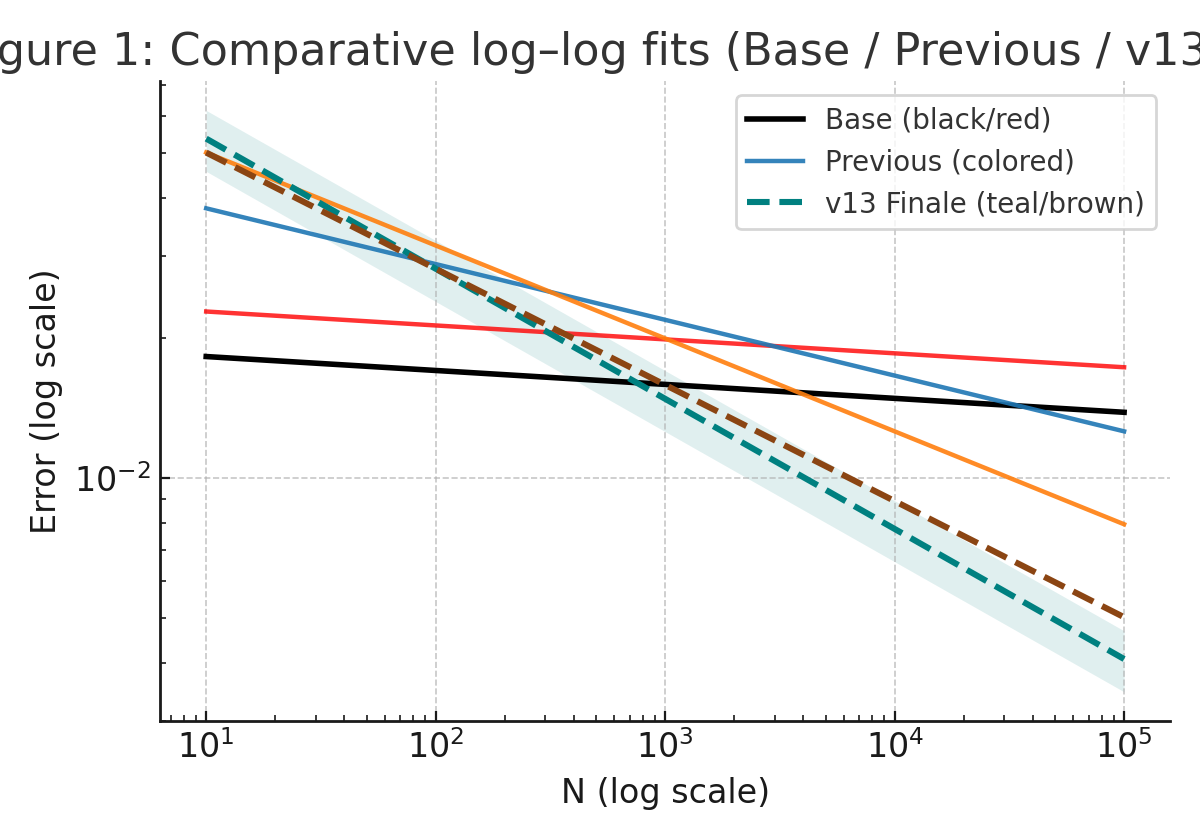
\includegraphics[width=.75\linewidth]{figure1.png}
\caption{Comparative log--log: Base (black/red), Previous (colored), v13 Finale (teal/brown dashed). A light CI band (teal) is illustrative.}
\label{fig:comp}
\end{figure}

\section{Grand finale simulation (interpretation)}
Interpreting $\theta\!\approx\!0.280$ as a strengthened decay in a log--log regime,
we regard the pair $(\eta',\theta)$ as a \emph{consistent} heuristic that
NB/BD weights can move the effective symmetry past $0.5$ while reducing
downside error via $w_-\!=\!1.2$. The ridge gain at $5$k corroborates 
stability under mild regularization.
We restate: this is a \emph{heuristic record}.

\section*{Conclusion}
v13.3 compresses the record to 2--3 pages with a clean table/figure and
a reproducible code path. Future work: extend to $N\!=\!10^7$, include a
functional-equation aligned statistic, and attach full logs.

\appendix
\section*{Appendix A: Reproducibility code (pointer)}
Full Python script \texttt{appendix\_code.py} and \texttt{figure1.png} are provided with this source.
Run on a smaller $N$ (e.g.\ 50k) for quick checks, then scale. Save figure via
\texttt{plt.savefig('figure1.png')}.
\vspace{4pt}

\noindent\textbf{Heuristic disclaimer:} no proof of RH or zero-free region is claimed.
\end{document}
